\chapter{Appendix}
\section{Definitions}
\begin{description}
\item[Record:] The data stored in a \ac{DHT} under one key (or \emph{record
ID}). Also contains a timestamp giving the time of last change.
\item[Peer:] One participant of the system, has one unique \emph{ID}; commonly
called \emph{node} in the context of \acp{DHT}.
\item[ID, Peer ID:] A bit string the length of which is fixed and prescribed by
the \emph{rules of the system}. Uniquely identifies a peer.
\item[Record ID:] A bit string of the same length as a \emph{peer ID}. Uniquely
identifies the record belonging to the peer with the same ID. Technically the
key of the record, but the word ID is used to stress that it's of the same kind
as a peer ID.
\item[Reachability information:] The abstract notion of information stored in
records in the \ac{DHT} that is sufficient to communicate with a peer. More
concretely, an IP address.
\item[Target ID:] A bit string that is the subject of a \emph{query}. Its length
is less than or equal to that of a \emph{peer ID}. If less, the query is asking
for any peer whose ID starts with the target ID.
\item[Matching an ID:] Two ID's match iff one is a prefix of the other. E.g., a
\emph{target ID} matches a \emph{peer ID} (or a \emph{record ID}) if the target
ID is a prefix of the peer ID, i.e., the peer ID is a valid response for a query
asking for the target ID.
\item[Overlap $o(a, b)$:] The length of the longest common prefix of two bit
strings. Defined in Section~\ref{sec:desc_querying}.
\item[Being closer to an ID:] ID A is closer to ID X than ID B iff the overlap
of A and X is greater than that of B and X.
\item[Routing prefix:] The prefix of a \emph{peer ID} of a length that is equal
for all peers and prescribed by the \emph{rules of the system}. Determines which
\emph{sync group} a peer is in.
\item[Being responsible for a routing prefix:] A peer is responsible for a
routing prefix iff the routing prefix is a prefix of his ID, i.e. he is in the
\emph{sync group} associated with that routing prefix.
\item[Sync group:] A group of peers who are \emph{responsible for} the same
routing prefix. Maintain contact in order to exchange updates regarding the
records they store.
\item[Sync peer:] Peers A and B are sync peers of one another iff they are in
the same \emph{sync group}.
\item[Authority (with regards to a sync group/peer):] Sync groups or peers are
an authority, or authoritative, for their routing prefix because they are
responsible for keeping current with updates to its records.
\item[Query group:] A group of peers that may send each other \emph{queries}.
Maintain contact in order to track each other's reputation within the group.
\item[Query peer:] Peers A and B are query peers iff they are in the same
\emph{query group}.
\item[Subprefix:] A prefix of a \emph{routing prefix} where
the last bit is flipped. Each peer has a number of subprefixes equal to the
length of the routing prefix.
\item[Serving a subprefix:] Peer A serves subprefix P for peer B iff P is a
subprefix of B's and a prefix of A's routing prefix.
\item[Subprefix coverage:] The state of a peer's ability to forward queries,
which is dependent on having query peers serving subprefixes. The subprefix
coverage is complete iff, for each of his subprefixes, the peer has a query peer
serving it.
\item[Request (for a target ID):] External stimulus to the system prompting it
to resolve the target ID. Simulates interaction of e.g. a user with the protocol
stack. Not to be confused with a \emph{query}.
\item[Query (for a target ID):] Message sent from one peer (the querying peer)
to another (the recipient) requesting the \emph{record} for the target ID.
\item[Response, fail response:] Message sent from one peer (the responding peer)
to another to answer a \emph{query}. The responder may claim to have included
the correct record, making the response successful, or that he is unable to
resolve the correct record, making it a fail response.
\item[Usefulness:] A measure of how useful or important peer B is to peer A to
complete subprefix coverage. Based on the length of subprefix B can serve for A,
but can also incorporate the trust in A or how many other peers A knows also
serving that subprefix. Used by B to estimate how many queries he is likely to
get from A, or from an entire group of peers (see
Section~\ref{sec:desc_usefulness}).
\item[Reputation:] A non-negative, real number stored in every query group for
each of its members. Earned by peers for better quality of service.
\item[Reputation record:] The copy of all of a peer's query peers' reputation
stored locally.
\item[Reputation decay:] Process that subtracts reputation from every peer in a
query group at a steady rate.
\item[Reward, penalty:] A change in a peer's reputation respectively increasing
or decreasing it.
\item[Cooperative action:] An action performed by a peer that warrants a reward.
\item[Defecting action:] An action performed by a peer that warrants a penalty.
\item[Tremble:] A defecting action that was not intended by the peer, but e.g.
caused by a congested network.
\item[Cooperation confirmation:] A signed statement given to another peer
confirming that he performed a cooperative action.
\item[Reputation attenuation:] A reduction of the magnitude of rewards that
takes effect once a peer's reputation passes a minimum (see
Section~\ref{sec:attenuation}).
\item[Raw and effective reputation:] Reputation before and after
\emph{reputation attenuation} takes effect.
\item[Recursive query:] A query in which the recipient performs all further
querying on behalf of the sender and returns the final result.
\item[Iterative query:] A query in which the recipient only indicates the next
suitable peer to query, the sender must perform the query himself. Requires
\emph{query vouchers} to provide a good level of service (see
Section~\ref{sec:desc_recursive_vs_iterative}).
\item[Query voucher:] A one-time-use statement entitling one peer to the level
of service of another. Used for iterative queries.
\item[Routing loop:] Failure in looking up a record in the \ac{DHT} caused by at
least one peer in the chain of queries forwarding the query to a peer who is not
\emph{closer to} the \emph{target ID}. The query is sent back to peers who
originally sent it. See also Section~\ref{sec:selection}.
\item[Entry peer:] A peer who is a member of a query group and facilitates the
joining of another peer into that group.
\item[Recursive query problem:] An issue in which a peer's low reputation in one
query group negatively affects his reputation in another (see
Section~\ref{sec:desc_rec_query_prob}).
\item[Penalty delay:] The delay that is deliberately imposed before responding
to a query to penalize the querying peer.
\item[Penalty threshold reputation (short: penalty threshold):] The minimum
reputation a peer must have in order for the penalty delay to be 0.
\item[Saturation reputation, being saturated:] The amount of reputation at which
a peer considers himself to have enough and isn't motivated to do work in order
to earn more.
\item[Broadcast:] The spreading of the same message to all peers in some group.
Explicitly \textbf{not} necessarily an actual broadcast on the network layer,
may also be executed as multiple unicasts. The term is used for simplicity of
discussion.
\end{description}

\section{Default Settings}
\label{sec:app_default_settings}
Table~\ref{tab:default_settings} lists the values for a selection of the most
important parameters in the default settings. Below, some of the ones that
aren't quite self-explanatory are explained more closely. All possible
parameters are available in the code repository in the commented default
settings file \texttt{simulation/default.settings}, relative to the repository
root (TODO check).

\begin{longtable}{|l|l|}
\hline
\rowcolor{slightgray} \T Key & Value \B\\
\hline
\cellcolor{slightgray}\T \texttt{rng\_seed} & 5803379951609632196 \B\\
\hline
\cellcolor{slightgray}\T \texttt{peer\_batches} & \texttt{[(0, 64, \{\})]} \B\\
\hline
\cellcolor{slightgray}\T \texttt{num\_random\_introductions} & 8 \B\\
\hline
\cellcolor{slightgray}\T \texttt{even\_sync\_groups} & \texttt{False} \B\\
\hline
\cellcolor{slightgray}\T \texttt{initial\_reputation} & 0 \B\\
\hline
\cellcolor{slightgray}\T \texttt{force\_one\_group} & \texttt{False} \B\\
\hline
\cellcolor{slightgray}\T \texttt{ensure\_non\_empty\_sync\_groups} & \texttt{True} \B\\
\hline
\cellcolor{slightgray}\T \texttt{id\_length} & 16 \B\\
\hline
\cellcolor{slightgray}\T \texttt{prefix\_length} & 4 \B\\
\hline
\cellcolor{slightgray}\T \texttt{ignore\_non\_existent\_subprefixes} & \texttt{False} \B\\
\hline
\cellcolor{slightgray}\T \texttt{transmission\_delay} & 0.1 \B\\
\hline
\cellcolor{slightgray}\T \texttt{successful\_query\_reward} & 1 \B\\
\hline
\cellcolor{slightgray}\T \texttt{failed\_query\_penalty} & -1 \B\\
\hline
\cellcolor{slightgray}\T \texttt{timeout\_query\_penalty} & -2 \B\\
\hline
\cellcolor{slightgray}\T \texttt{no\_penalty\_reputation} & 10 \B\\
\hline
\cellcolor{slightgray}\T \texttt{reward\_attenuation $\rightarrow$ type} & \texttt{exponential} \B\\
\hline
\cellcolor{slightgray}\T \texttt{reward\_attenuation $\rightarrow$ exponent} & 0.35 \B\\
\hline
\cellcolor{slightgray}\T \texttt{reward\_attenuation $\rightarrow$ coefficient} & 1 \B\\
\hline
\cellcolor{slightgray}\T \texttt{reward\_attenuation $\rightarrow$ lower\_bound} & 10 \B\\
\hline
\cellcolor{slightgray}\T \texttt{reward\_attenuation $\rightarrow$ upper\_bound} & 15 \B\\
\hline
\cellcolor{slightgray}\T \texttt{reputation\_buffer} & 4 \B\\
\hline
\cellcolor{slightgray}\T \texttt{query\_peer\_selection} & \texttt{overlap\_rep\_sorted} \B\\
\hline
\cellcolor{slightgray}\T \texttt{query\_sync\_for\_subprefixes} & \texttt{False} \B\\
\hline
\cellcolor{slightgray}\T \texttt{uncovered\_subprefix\_interval} & 10 \B\\
\hline
\cellcolor{slightgray}\T \texttt{min\_desired\_query\_peers} & 2 \B\\
\hline
\cellcolor{slightgray}\T \texttt{max\_desired\_group\_size} & 16 \B\\
\hline
\cellcolor{slightgray}\T \texttt{query\_timeout} & 2 \B\\
\hline
\cellcolor{slightgray}\T \texttt{expect\_penalties} & \texttt{True} \B\\
\hline
\caption{Default values of a selection of settings.}
\label{tab:default_settings}
\end{longtable}

\begin{description}
\item[\texttt{peer\_batches}] A list of tuples \texttt{(time, number\_of\_peers,
settings)} that allows to add peers at different times and with individual
settings.
\item[\texttt{num\_random\_introductions}] Upon initialization, each peer is
introduced to a random sample of peers. This is the size of that sample.
\item[\texttt{even\_sync\_groups}] If \texttt{True}, initialization will take
care to make all sync groups the same size. This can be helpful in ruling out
unevenly sized sync groups as the cause of some observed effect.
\item[\texttt{force\_one\_group}] If \texttt{True}, all peers will be forced
into one query group. Can be helpful e.g. to rule out the recursive query
problem as the cause of some effect.
\item[\texttt{ensure\_non\_empty\_sync\_groups}] If \texttt{True},
initialization takes care that each sync group contains at least one peer.
\item[\texttt{prefix\_length}] Length of the routing prefix, which is just
called prefix in the simulation.
\item[\texttt{ignore\_non\_existent\_subprefixes}] If \texttt{True}, peers make
use of global information they are given in the beginning in order to not query
for subprefixes for which there doesn't exist a peer (i.e. the sync group is
empty) when they are completing their subprefix coverage. This is useful in
preventing ongoing querying for IDs that will never lead to a successful
response.
\item[\texttt{no\_penalty\_reputation}] The penalty threshold reputation.
\item[\texttt{reputation\_buffer}] The amount of reputation above the penalty
threshold peers need to have in order to consider themselves reputation
saturated.
\item[\texttt{query\_sync\_for\_subprefixes}] If \texttt{True}, peers will also
send queries to their sync peers (even if they are not query peers) when they
are completing their subprefix coverage.
\item[\texttt{uncovered\_subprefix\_interval}] Peers repeatedly check whether
they have complete subprefix coverage and send queries in order to complete it
if they don't. This is the time interval between checking.
\item[\texttt{expect\_penalties}] If \texttt{True}, peers expect to be penalized
when they perform a defecting action.
\end{description}


\begin{figure}[t]
\centering
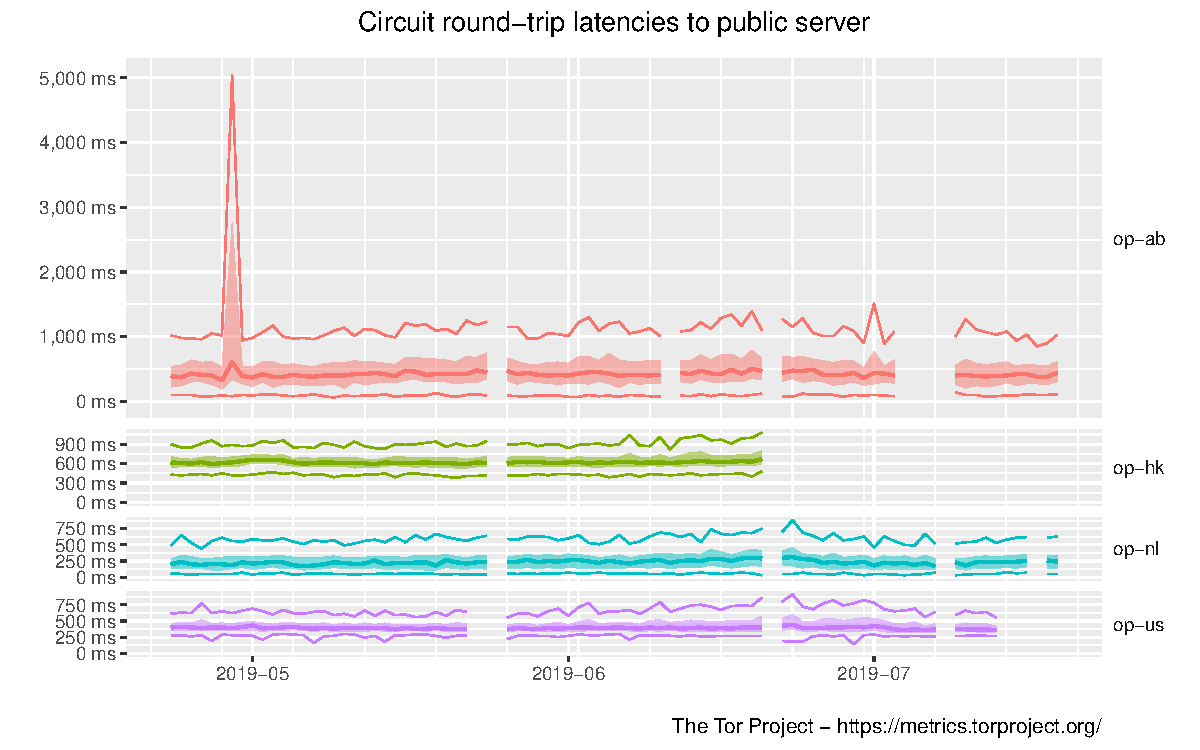
\includegraphics[width=1\columnwidth]{figures/onionperf-latencies-public-2019-04-23-2019-07-22}
\caption{Tor circuit RTTs from the Tor Project's metric site\cite{torperf}}
\label{fig:tor_rtt}
\end{figure}
